
In 2014 Goodfellow et al. proposed a framework for creating image generating models
using an adversarial loss function during training.
The aim of this loss function is for the generator model (G) to minimize the probability
for the discriminator (D) to recognize the output of G as fake, while the aim for D
is to minimize the probability of recognizing the output of G as real, while maximizing the
probability that D recognizes the ground truth as real.
In theory after training G it will then produce images that D cannot distinguish from the ground
truth.
C++ has long been a widely used language used for performance critical code, and with new
language standards more modern and fast abstraction tools have become available that make C++ an
attractive language to use in the modern software landscape.
In this paper I try to reimplement the model described in Generative Adversarial Networks in the
LibTorch C++ framework and evaluate the results.

\section{Introduction}\label{sec:introduction}
Image generation has long been an active field of study, but only in recent years have unsupervised
models been successful in creating high quality images after the advent of adversarial networks.
Previous techniques such as restricted Boltzmann machines, deep belief networks, stacked
convolutional auto-encoders, and deep generative stochastic networks have previously been used
for image generation to various levels of success, but generative adversarial networks produce
results better than any of those mentioned.
By training two networks in opposition to another the trained models can also serve two purposes:
one to generate data from a latent space, and another to detect fake images or videos (or so-called
"deep fakes")

\section{Methods}\label{sec:methods}
For the implementation, the C++ interface of PyTorch was used, along with png++ for data loading
and the C++17 standard utilities for multiprocessing.
The image dataset is loaded using a handwritten utility for loading image directories, sped up by
multiprocessing.
This image loading utility is capable of loading and processing about 15000 128x128 rgb images
per second, producing a transfer speed of up to approx. 500MB/s and a total loading time of the
2.1GB 128x128 FFHQ dataset of approx. 5 seconds on an AMD Ryzen 7 3800X with 8 cores, being
limited on CPU processing speed during conversion of data.
After loading, the dataset is normalized to have a mean of 0 and a standard deviation of 1.0, after
which it is processed into batches of 64 to 128 or more elements, depending on the problem and
the desired learning rate.

\subsection{MNIST}\label{subsec:mnist}
The discriminator model used for MNIST has a latent space of 100 variables, hidden layers of
sizes 256 and 128.
On the hidden layers of the discriminator model ReLU activation with dropout is used for each
layer, with a sigmoid activation layer as output.
Furthermore, the generator model consists of hidden layers of sizes 128, 256, and 512, with leaky
ReLU activation and dropout applied to each layer.
The RMSProp optimizer is used to train this model, with a learning rate of 0,0001.

\subsection{FFHQ}\label{subsec:ffhq}
The FFHQ (Flickr Faces High Quality) database is a database of high-quality images of faces
gathered from Flickr.
Because of computational constraints the chosen image size from the database is 128x128.
The images can be downloaded using the included download script in the dataset folder.
Two different models are tested for the FFHQ dataset: one fully connected model and one model 
based on convolutional layers, with different results.
Both models are optimized using the ADAM optimizer.

\subsubsection{Fully connected}
The fully connected model uses the same hidden layer composition as the MNIST model, with sizes
256 and 128 on the discriminator model, sizes 32, 64, 128, and 256 on the generator model, and a
latent space of 32 variables.

\subsubsection{Convolutional}
As an alternative for the fully connected model it is also possible to use a convolutional model.
This model consists of several convolutional layers and fully connected layers, allowing for both
positional dependent and positional independent information encoding.
The layers of the discriminator model are three convolutional layers of kernel size 5 and with
128, 256, and 256 output features, connected to fully connected layers of sizes 512, 256, and 64.
The generator has fully connected layers of 64 and 128, which is connected to deconvolutional
layers with a kernel size of 5, with 128, 64, 32, and 16 features.

\section{Results}\label{sec:results}

\begin{figure}[h!]
    \centering
    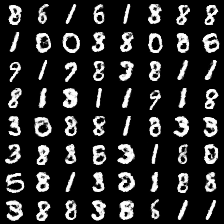
\includegraphics{media/output}
    \caption{Uncurated output after 1000 epochs}
    \label{fig:mnist_output}
\end{figure}

We can see that the output of the trained MNIST generator is fairly good, in earlier iterations
of training there is still some noise spikes apparent but with enough training these spikes are
eliminated.

\begin{figure}[h!]
    \centering
    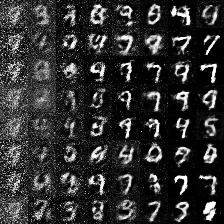
\includegraphics{media/training}
    \caption{Training process (from left to right, exponential training time)}
    \label{fig:mnist_training}
\end{figure}

In figure 2 the diminishing returns of training for longer can clearly be seen.
It is interesting to note that the generator model normally starts by replicating only one of the
digits in the dataset, after which it will start to diversify.

\begin{figure}[h!]
    \centering
    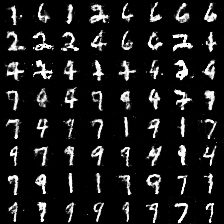
\includegraphics{media/interp}
    \caption{2D interpolation of latent space fully trained model}
    \label{fig:mnist_interp}
\end{figure}

Although the results are clustered, it is apparent in figure 3 that there are large nonlinearities
present in the latent space.
It can also be noted that although there are many regions that are similar in appearance in the
output layer which would indicate a generator model that is able to encode the entirety of the real
data distribution, there is often a lack of certain modalities that are far removed spatially
from other data points in the real dataset.
As an example of this, the number 2 in the MNIST dataset has few digits that are connected in the
data distribution, or it has few digits it can "morph into" so to say.
These modalities seem to be underrepresented because of a certain selection pressure, making
certain regions unreachable because of their disconnected nature.

\begin{figure}
    \centering
    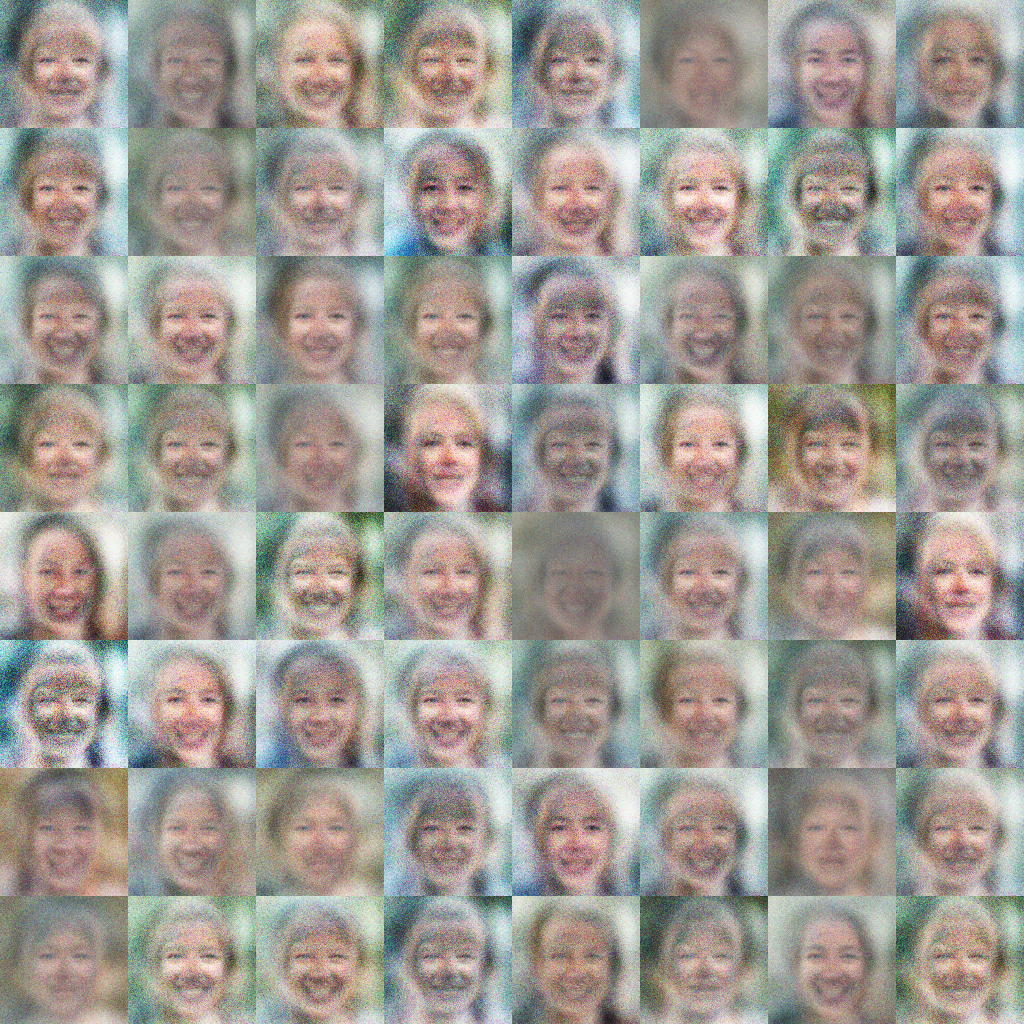
\includegraphics[width=\linewidth]{media/ffhq_fc}
    \caption{images created by the fully connected generator model trained on the FFHQ dataset}
    \label{fig:ffhq_fc}
\end{figure}

The fully connected model trained on the FFHQ dataset works fairly well, but because of the low
amount of learnable parameters it can only learn general information about the dataset.

\begin{figure}
    \centering
    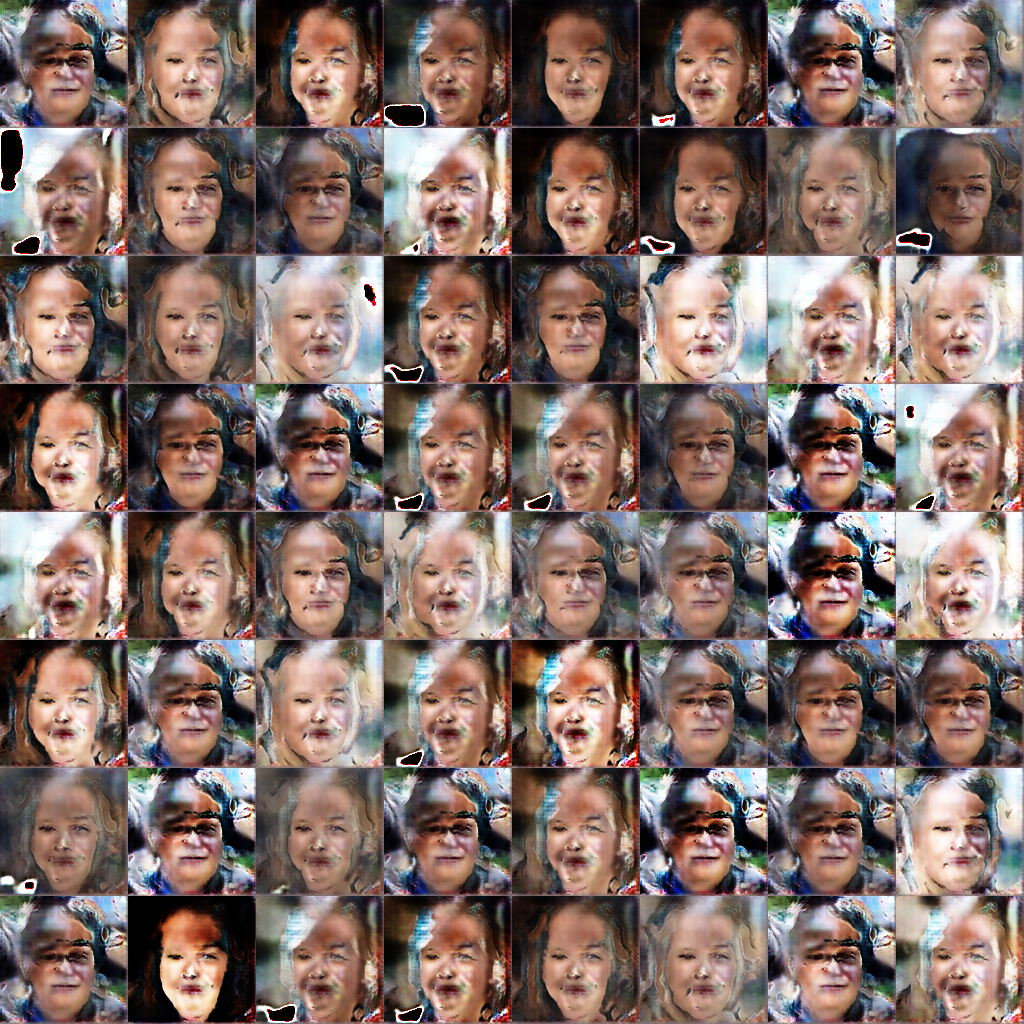
\includegraphics[width=\linewidth]{media/ffhq_cnn}
    \caption{images created by the convolutional FFHQ generator model}
    \label{fig:ffhq_cnn}
\end{figure}

The convolutional model seems to have issues with visual aberrations, possibly because of
incorrect value clipping in the png translation function.
Overall the output of the convolutional model is able to learn finer details and is able to
output more visually compelling images, but as a result the output is often disjointed with
various human features distributed in a picasso-like manner, recombining features from different
modalities into one semi-coherent image.

\begin{figure}
    \centering
    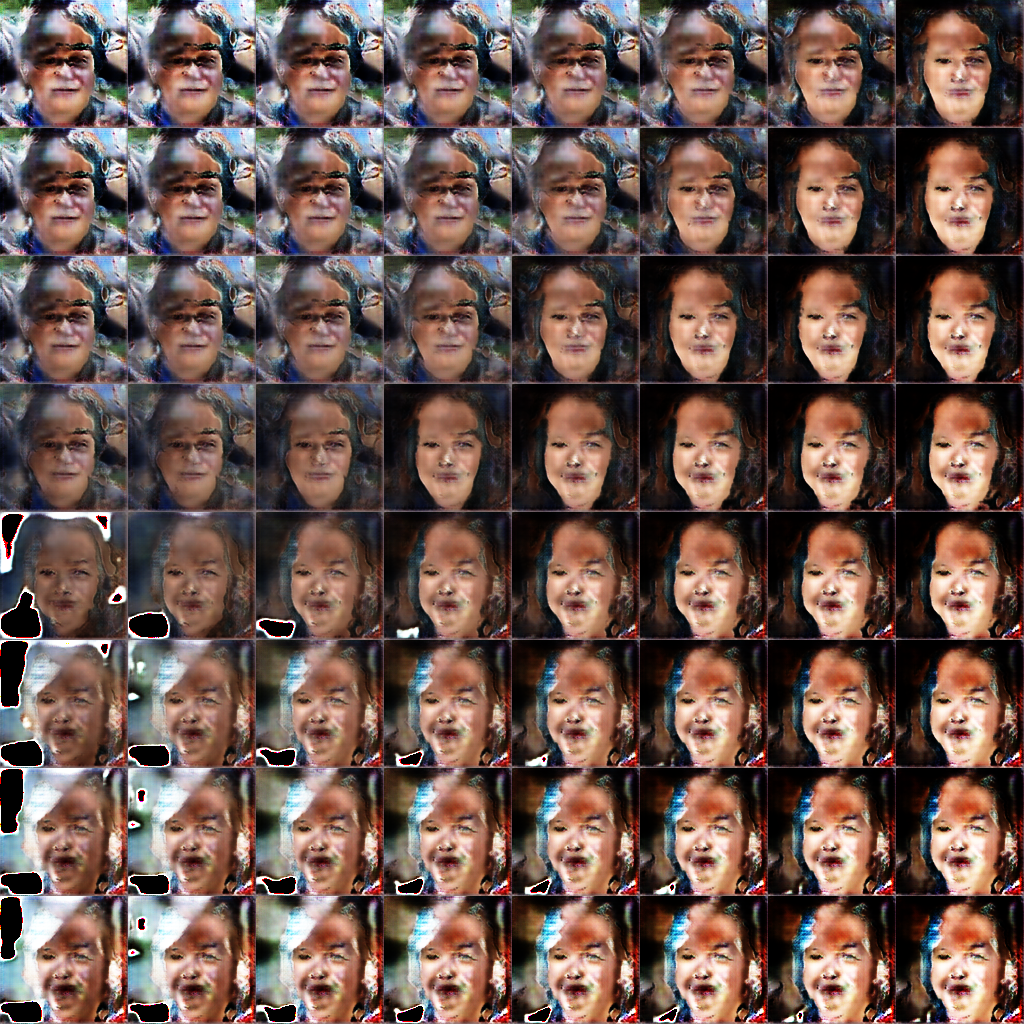
\includegraphics[width=\linewidth]{media/ffhq_cnn_interp}
    \caption{2D interpolation of the latent space of the FFHQ CNN generator model}
    \label{fig:ffhq_cnn_interp}
\end{figure}

In the interpolation of the latent space we can see that there is less variation than in the
MNIST example, indicating that there is probably a lack of parameters in the model to represent
all modalities.


\section{Discussion}\label{sec:discussion}
In the samples of the output several glyphs can be seen that do not look like numbers, or rather
look like a combination or in-between of different numbers.
These outputs can a result of high connectedness between two modes in the dataset, but it seems
more often it is because the backpropagation gradient is very shallow in those regions for the
discriminator, and thus also for the generator.
Of course this issue can be solved by simply training the model for longer.

As a general rule of thumb a slower learning rate comes with a better chance of convergence, this
can be done by lowering the learning rate parameter on the optimizer, but it is also possible to
increase the batch size, as a higher batch size means lower variance and thus smaller gradients
during the backwards pass.

Because of the learning rate problem, special care has to be taken when choosing the optimizer,
as some momentum based optimizers will automatically increase the learning rate to the point of
non-convergence.

Because of the underrepresented modes in the generator model, it might be prescient to have the
loss function put extra emphasis on those regions of the data that are not present or are
underrepresented.

The chioce of noise used in the latent space seemed to have a great effect on the results
produced, as the model was almost impossible to train using uniform noise, but using normally
distributed noise (with a standard deviation of 1) seemed to give much better and more stable
results.

\section{Bijlage}\label{sec:bijlage}
In deze bijlage worden alle beoordelingscriteria toegelicht.

\subsubsection{De student kan vision-algoritmes implementeren ten behoeve van een geselecteerde
    Vision taak.}
Het algoritme is geimplementeerd zoals beschreven in de originele paper, en andere algoritmes
voor data laden en opslaan zijn geimplementeerd.
\subsubsection{De student kan papers uit de wetenschappelijke literatuur over computer vision lezen,
    begrijpen, en omzetten naar code.}
Zie vorig punt, het originele paper is gerepliceerd, behalve de Gaussian Parzen window sinds ten
eerste dit een complex algoritme is en er geen goede indicatie is gegeven hoe het geimplementeerd
is in de originele paper, en ten tweede omdat deze metric alleen nuttig is in vergelijking met
andere modellen, en dat valt buiten de scope van dit project.
\subsubsection{De student kan een opdracht analyseren en op basis hiervan het benodigde werk
    (waaronder het implementeren en verdelen en plannen).}
De planning is aan het begin van het project gemaakt, en sinds dien is er ten alle tijden uiterst
een aantal dagen achterstand geweest; de planning is correct gemaakt voor de tijd die beschikbaar was.
\subsubsection{De student kan omgaan met software oplossingen voor versiebeheer (GIT) en kan deze
    software inzetten voor het ontwikkelen van code.}
Alle code en verandering zijn correct bij gehouden in GIT.
\subsubsection{De student kan een experiment opzetten en uitvoeren om aan te tonen hoe de
    geïmplementeerde vision-methode werkt, hoe effectief (zowel in kwaliteit als in snelheid)
    deze methode en implementatie is en waar grenzen liggen van de gekozen methode en implementatie}
De originele methode is geimplementeerd en de resultaten zijn in dit document op genomen, met
goede resultaten op de MNIST dataset, en acceptabele resultaten op de FFHQ dataset.
\subsubsection{De student kan een rapport schrijven om het gekozen en uitgevoerde experiment te
    beschrijven, de resultaten te beschrijven en conclusies te trekken.}
In deze paper zijn de methoden uitgebreid beschreven en de resultaten geanalyseerd in de
bijbehorende hoofdstukken.
\subsubsection{De student kan een zelf-opgezet experiment uitvoeren en de resultaten op
    gestructureerde wijze verzamelen.}
Het experiment is uitgevoerd en de experimenten verwerkt.
